\documentclass[a4paper,11pt,notitlepage,fullpage]{article}
%\documentclass{report}

\usepackage{fullpage}
\usepackage[utf8]{inputenc}
%\usepackage[ngerman]{babel}
%\usepackage[english]{babel}
\usepackage{amsmath}
\usepackage{amssymb}
\usepackage{latexsym}
\usepackage{mathtools}
\usepackage{listings}
\usepackage{bbm}
%\usepackage{algorithm}
%\usepackage{algpseudocode}
\usepackage{graphicx}
\usepackage{booktabs}
\usepackage{hhline}
\usepackage{amsthm}
\usepackage{cite}
\usepackage{wrapfig}
\usepackage{hyperref}
\usepackage{titling}
\usepackage{color}

\setlength{\droptitle}{-60pt}

\newcommand{\R}{\mathbb R}
\newcommand{\p}{\mathbb P}
\newcommand{\pp}[1]{\mathbb P\left[#1\right]}
\newcommand{\E}[1]{\mathbb E\left[#1\right]}
\newcommand{\V}{\mathbb V}
\newcommand{\Vv}[1]{\mathbb V\left[#1\right]}
\newcommand{\Cov}[1]{\mathbb Cov\left[#1\right]}
\newcommand{\F}{\mathcal{F}}
\newcommand{\ind}{\mathbbm{1}}
\newcommand{\indd}[1]{\mathbbm{1}_{#1}}
\newcommand{\norm}[2]{\left|\left|{#1}\right|\right|_{#2}}
\DeclareMathOperator*{\limm}{l.\hspace{-0.18em}i.\hspace{-0.19em}m}
\DeclareMathOperator*{\spann}{span}

\begin{document}
\author{Florian Bogner \& Alexander Palmrich}
\title{Stochastische Prozesse - Übung 11}
\maketitle

\begin{enumerate}
\setcounter{enumi}{46}

%%für ein Bild das copy-pasten und reinkommentieren
%\begin{figure}[h!]
%\centering
%\includegraphics[width=0.9\textwidth]{gfx/bildname.png}
%\label{fig1}
%\caption{TODO Beschreibung des Bildes}
%\end{figure}

%01
\item Laut Folie 129 ist das AR-Polynom $q(z) := 1 - a z^4 \neq 0$ für $|z| \leq 1$ da $|a| < 1$. Damit ist die Stabilitätsbedingung erfüllt. Wir tanzen die Vorlesungsfolie 110 nach: 
\begin{align*}
x_t &= a x_{t-4} + \epsilon_t \\
&= a^2 x_{t-8} + a \epsilon_{t-4} + \epsilon_t \\
&= a^3 x_{t-12}+ a^2 \epsilon_{t-8} + a \epsilon_{t-4} + \epsilon_t \\
&= \vdots \\
&= \limm_{k \to \infty}\left( a^k x_{t-4k} + \sum_{j=0}^{k-1}a^j \epsilon_{t-4j} \right) \\
&= 0 + \sum_{j\geq0} a^j \epsilon_{t-4j}
\end{align*}
Damit haben wir unserern Lösungskandiaten gefunden. Probe:
\begin{align*}
x_t = \sum_{j\geq0} a^j \epsilon_{t-4j} = \epsilon_t + a\sum_{j=0}^{\infty} a^j \epsilon_{t-4-4j} = a x_{t-4} + \epsilon_t
\end{align*}
Hurra. ACF:
\begin{align*}
\gamma(k) &= \langle x_t, x_{t-k} \rangle \\
&= \sum_{j\geq0} \sum_{i\geq0} \langle a^j \epsilon_{t - 4j}, a^{i-k} \epsilon_{t - k - 4i}\rangle \\
&= \sum_{j\geq0} \sum_{i\geq0} a^{j+i-k} \langle \epsilon_{t - 4j}, \epsilon_{t - k - 4i}\rangle \\
&= \sum_{j\geq0} \sum_{i\geq0} a^{j+i-k} \delta_{4j}^{k+4i} \sigma^2 \\
&= \begin{cases}
0 & k \neq 0 \mod 4 \\
\sigma^2 \sum_{j\geq0} a^{2j-k} & k = 0 \mod 4 \\
\end{cases} \\
&= \begin{cases}
0 & k \neq 0 \mod 4 \\
\sigma^2 \frac{a^{-|k|}}{1 - a^2} & k = 0 \mod 4 \\
\end{cases} \\
\end{align*}

\begin{figure}[h!]
\centering
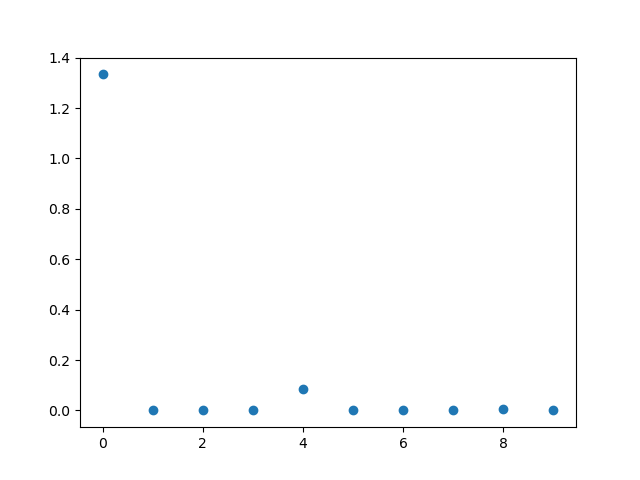
\includegraphics[width=0.9\textwidth]{gfx/47_fig.png}
\label{fig1}
\caption{ACF vom $x_t$ (unter der Annahme $a= 0.5$ und $\sigma^2 = 1$)}
\end{figure}


%02
\item Das AR-Polynom von $x_t = 0.1 x_{t-1} - 0.2 x_{t-2} + 0.3 x_{t-3} + \epsilon_t$ ist $$q(z) = 0.1 z - 0.2 z^2 + 0.3 z^3 + 1$$.
Wir wenden die umgekehrte Dreiecksungleichung an und schätzen $|z| \leq 1$ ab:
$$|q(z)| \geq -(0.1 + 0.2 + 0.3) + 1 = 0.4$$
Damit hat $q(z)$ keine Nullstellen in der Einheitskreisscheibe und die Stabilitätsbedingung ist erfüllt. Mit etwas Python-Code geht das $\bar b$ berechnen ganz schnell:
\begin{verbatim}
l = 6
p = 3
a = (0, +0.1, -0.2, +0.3)
b = [0]*l

b[0] = 1
for k in range(1, l):
    b[k] = sum([a[i] * b[k-i] for i in range(1, p+1) if k-i >= 0])

print("\nb = ", b)

###############################
sigmasq = 1
import numpy as np
from scipy import linalg as lin
from itertools import product

k = 6
A = np.eye(k)
for i, j in product(range(k), range(k)):
    if 0 < i+j <= p:
        A[i,j] -= a[i+j]
    if j > 0 and 0 < i-j <= p:
        A[i,j] -= a[i-j] 
b = np.array([sigmasq]+[0]*(k-1))
y = np.linalg.solve(A, b)

print("\nA := ", A)
print("\ngamma = ", y)
\end{verbatim}
Das liefert uns das Erbebnis:
\begin{verbatim}
b =  [1, 0.1, -0.19, 0.261, 0.0941, -0.09978999999999999]

A :=  [[ 1.  -0.1  0.2 -0.3  0.   0. ]
 [-0.1  1.2 -0.3  0.   0.   0. ]      
 [ 0.2 -0.4  1.   0.   0.   0. ]      
 [-0.3  0.2 -0.1  1.   0.   0. ]      
 [ 0.  -0.3  0.2 -0.1  1.   0. ]
 [ 0.   0.  -0.3  0.2 -0.1  1. ]]

gamma =  [ 1.1402027   0.04222973 -0.21114865  0.3125      0.08614865 -0.11722973]
\end{verbatim}


%03
\item Mit der Funktion aus Bsp. 39 ist der schwerste Teil schon gemacht:
\begin{verbatim}
import numpy as np
from scipy import linalg as lin

gamma = np.array((8.952,
                  7.870,
                  7.083,
                  6.562,
                  6.036,
                  5.537,
                  5.086,
                  4.673,
                  4.292,
                  3.942))

def prognose(h, k):
    GAMMA = lin.toeplitz(gamma[0:k])
    c = gamma[h:h+k] @ lin.inv(GAMMA)
    err = gamma[0] - c @ GAMMA @ c.T
    return c, err

for p in range(1, 10):
    a, err = prognose(1, p)
    print(f"{p=}: {err=}")
    print(f"{a=}\n")
\end{verbatim}
resultiert im Output:
\begin{verbatim}
p=1: err=2.033222073279715
a=array([0.87913315])

p=2: err=2.0199579592870975
a=array([0.80812612, 0.08076937])

p=3: err=1.999679919038699
a=array([ 8.00033512e-01, -2.00035381e-04,  1.00194025e-01])

p=4: err=1.99967948648895
a=array([ 8.00080111e-01, -2.00128416e-04,  1.00566114e-01, -4.65090837e-04])

p=5: err=1.9996794142110002
a=array([ 8.00080199e-01, -2.19247822e-04,  1.00566152e-01, -6.17200292e-04,
        1.90117781e-04])

p=6: err=1.999679385494888
a=array([ 8.00080177e-01, -2.19173860e-04,  1.00554100e-01, -6.17174019e-04,
        9.42404041e-05,  1.19834708e-04])

p=7: err=1.9996792602099633
a=array([ 8.00080147e-01, -2.19197449e-04,  1.00554255e-01, -6.42343195e-04,
        9.42952643e-05, -8.04292185e-05,  2.50304822e-04])

p=8: err=1.9996790975075136
a=array([ 8.00080218e-01, -2.19220391e-04,  1.00554282e-01, -6.42526420e-04,
        1.22977786e-04, -8.04917434e-05,  4.78523071e-04, -2.85244233e-04])

p=9: err=1.9996790877197732
a=array([ 8.00080198e-01, -2.19186913e-04,  1.00554276e-01, -6.42517816e-04,
        1.22932833e-04, -7.34567899e-05,  4.78507734e-04, -2.29269222e-04,
       -6.99617490e-05])
\end{verbatim}
Wir sehen dass sich nach $p=3$ der Fehler nicht wirklich ändert und die hinzukommenden Koeffizient kleiner sind als die Genauigkeit, mit der uns $\gamma$ gegeben wurde. Der wahre Prozess ist also ein $AR(3)$-Prozess mit $x_t = 0.8x_{t-1} - 0.1x_{t-3}$ und $\sigma^2 = 2$.


%04
\item bla
\begin{enumerate}
%a
\item a
\begin{align*}
\end{align*}

%b
\item b
\begin{align*}
\end{align*}
\end{enumerate}



\end{enumerate}



\end{document}
